% IDI S26 — BER+ Board Room — Final Team Presentation (camera-ready, 2–4 pages)
% Compile: node copy-figures.mjs && pdflatex idi-s26-final-submission.tex (twice)

\documentclass[10pt,a4paper]{article}
\usepackage[utf8]{inputenc}
\usepackage[T1]{fontenc}
\usepackage[margin=1.75cm]{geometry}
\usepackage{graphicx}
\usepackage{booktabs}
\usepackage{hyperref}
\usepackage{parskip}
\usepackage{caption}
\usepackage{subcaption}
\usepackage{xcolor}

\hypersetup{colorlinks=true, linkcolor=blue!70!black, urlcolor=blue!70!black}
\newcommand{\demourl}{\url{https://ber-board-room.vercel.app/}}
\newcommand{\berhub}{\textbf{BER+ Board Room}}
\newcommand{\sectionrule}{\vspace{0.25em}{\color{black!20}\hrule height 0.4pt}\vspace{0.45em}}

\graphicspath{{figures/}}
\setlength{\parskip}{0.4em}
\setlength{\parindent}{0pt}
\captionsetup{font=small,skip=4pt}
\hyphenation{Data-driven}

\begin{document}

\begin{center}
  {\LARGE \berhub{}}\\[0.3em]
  {\large \mbox{Data-driven} transparency \textperiodcentered\ ecosystem coordination probe}\\[0.45em]
  {\normalsize Tian Shao \textperiodcentered\ Yushu Qin \textperiodcentered\ Yi Li}\\[0.15em]
  {\small XU University of Applied Sciences \textperiodcentered\ IDI S26 \textperiodcentered\ June 2026}\\[0.35em]
  {\small\textbf{Live prototype:} \demourl}
\end{center}
\sectionrule

\section*{1.\ Course objective \& problem}
\textbf{Objective (not a final strategy).}
We explore opportunities, challenge assumptions, and offer \textit{actionable impulses} for BER+ --- not a finished regional strategy.

\textbf{The corridor pain.}
Land, grid, logistics, and programme milestones sit in PDFs and member decks --- never on one map. Members see their own sites but not what is \textit{in play} nearby.

\textbf{Our story.}
\textbf{Data-driven transparency}: a neutral BER+ briefing platform with labelled indicative evidence on one map before site visits and contracts.

\section*{2.\ The Board Room prototype}
\berhub{} is a live web probe: MapLibre corridor map, 14 Mitglieder, OSM Intel, Pilot-1 timeline, stakeholder matching, bilingual welcome, guided walkthrough.

\begin{figure}[htbp]
  \centering
  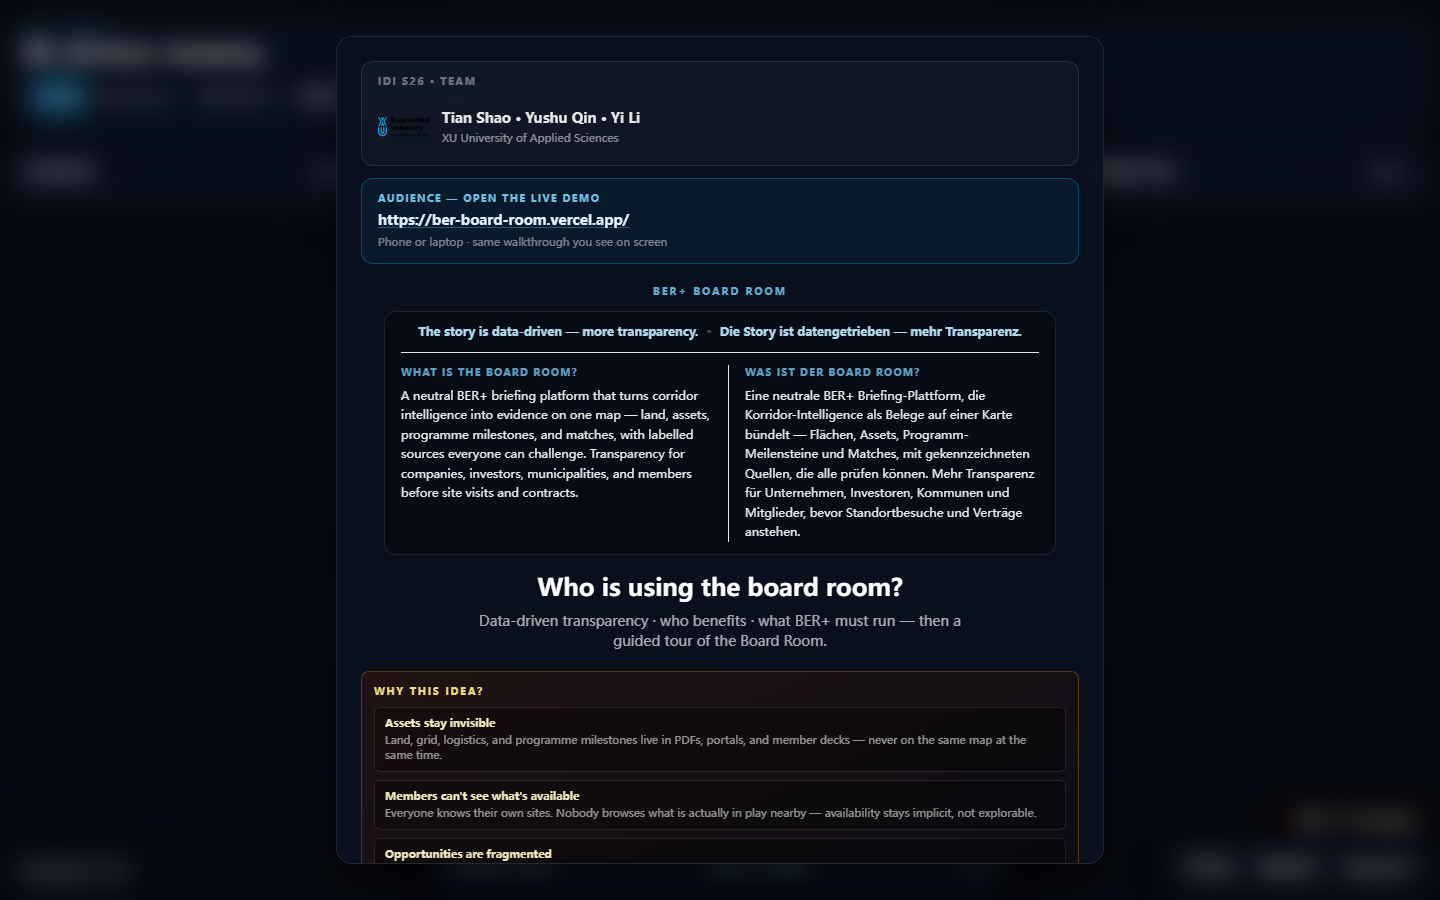
\includegraphics[width=\linewidth,keepaspectratio]{fig-session-picker.png}
  \caption{Welcome --- team, audience URL, bilingual Board Room explainer (Playwright, desktop).}
\end{figure}

\begin{figure}[htbp]
  \centering
  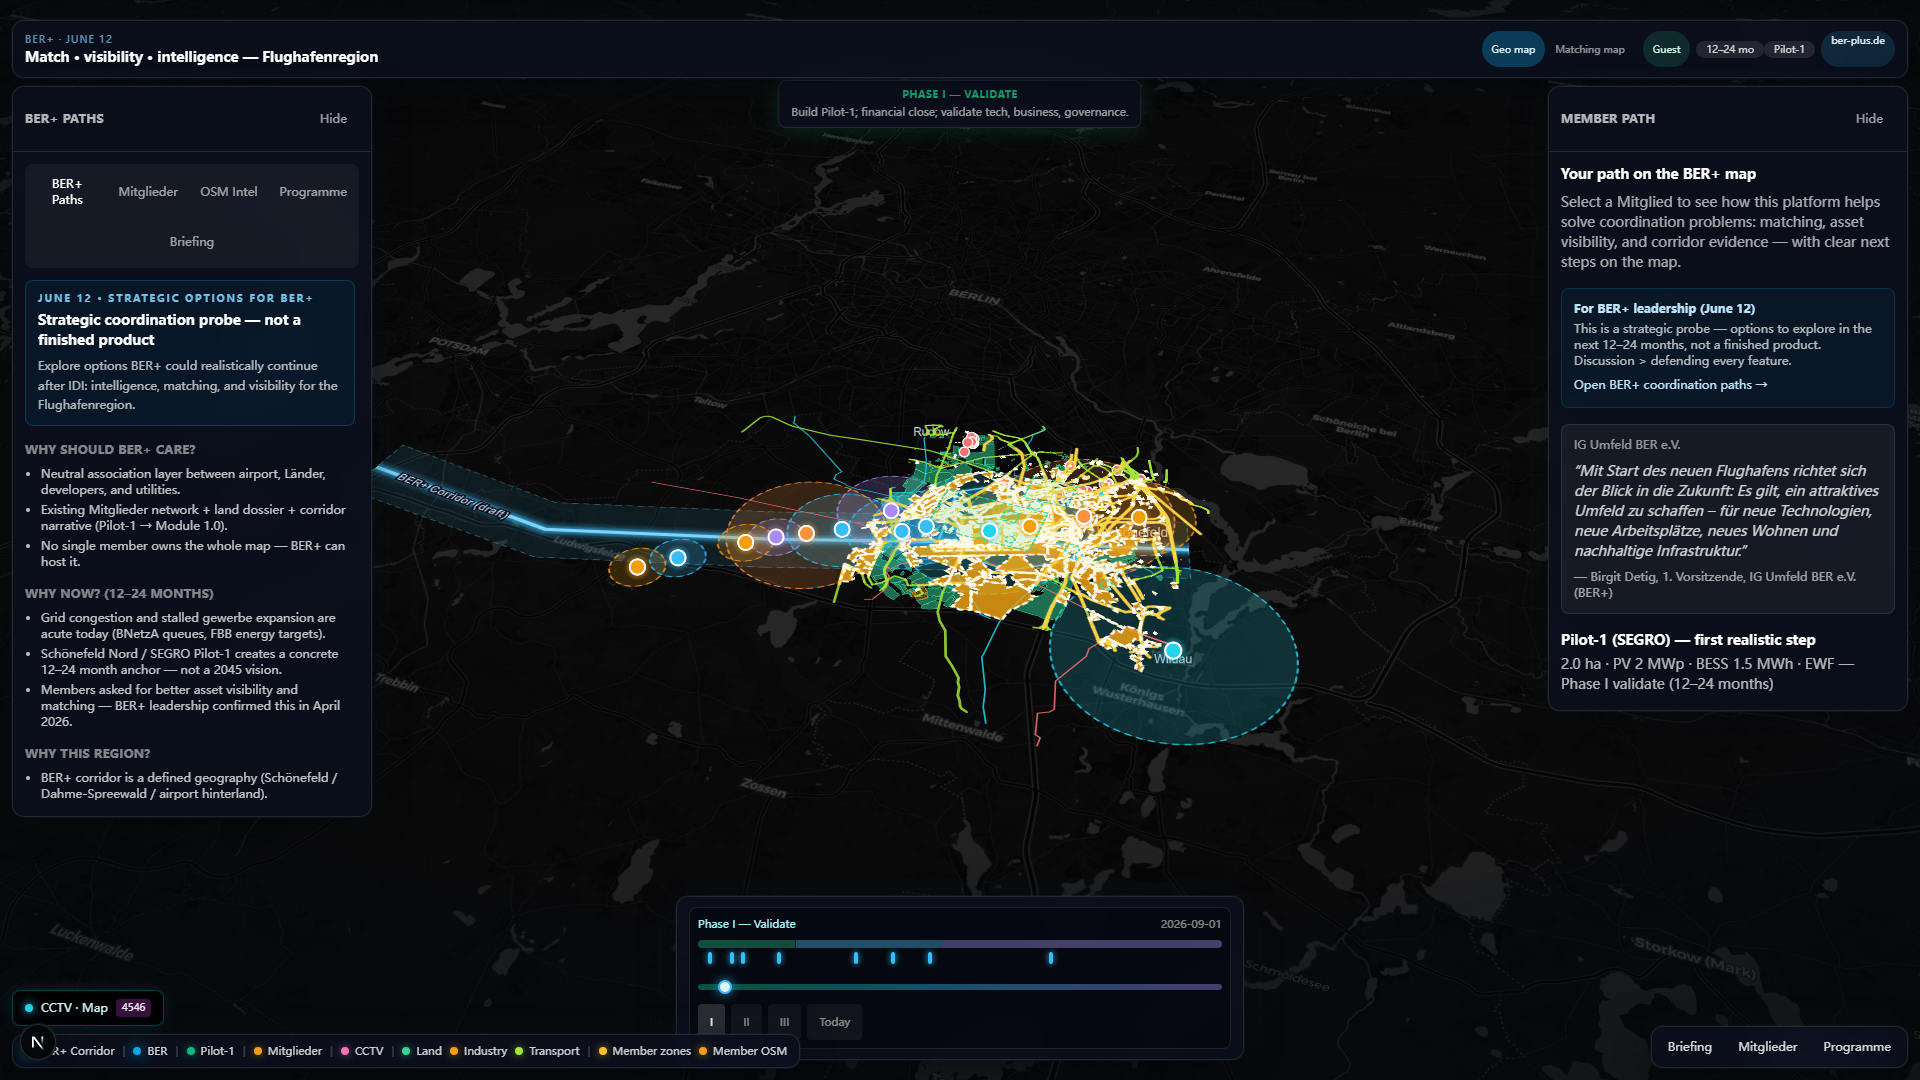
\includegraphics[width=\linewidth,height=0.34\textheight,keepaspectratio]{fig-war-room-overview.png}
  \caption{Board Room map --- corridor ribbon, Pilot-1, Mitglieder zones, programme timeline.}
\end{figure}

\textbf{Three demo walkthroughs} on \demourl:
\begin{itemize}
  \setlength{\itemsep}{0.15em}
  \item \textbf{Company} --- OSM land, developer focus, matching intro.
  \item \textbf{Investor} --- Mitglieder density, hectares, benchmark teleport.
  \item \textbf{Municipality} --- briefing + infrastructure layers (indicative only).
\end{itemize}

\begin{figure}[htbp]
  \centering
  \begin{subfigure}[t]{0.32\textwidth}
    \centering
    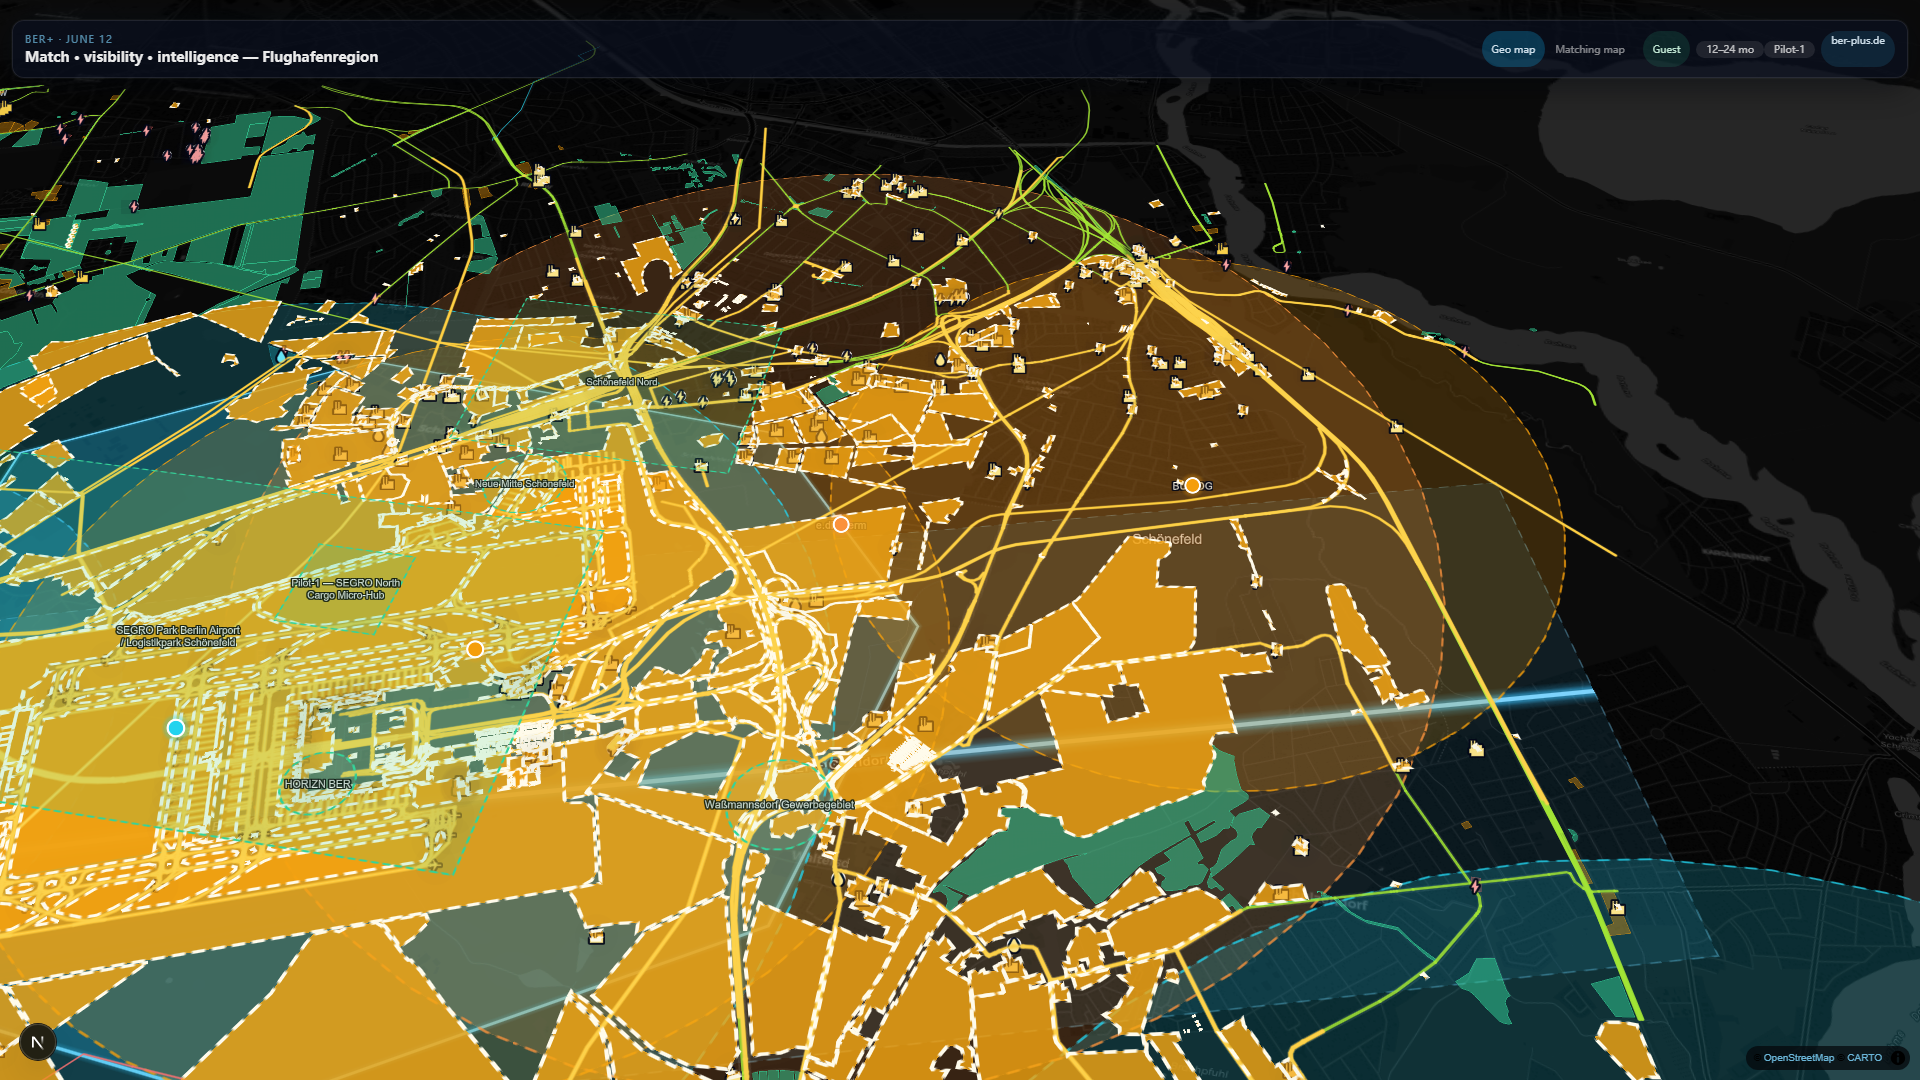
\includegraphics[width=\linewidth,height=0.2\textheight,keepaspectratio]{fig-osm-intel.png}
    \caption*{OSM Intel}
  \end{subfigure}\hfill
  \begin{subfigure}[t]{0.32\textwidth}
    \centering
    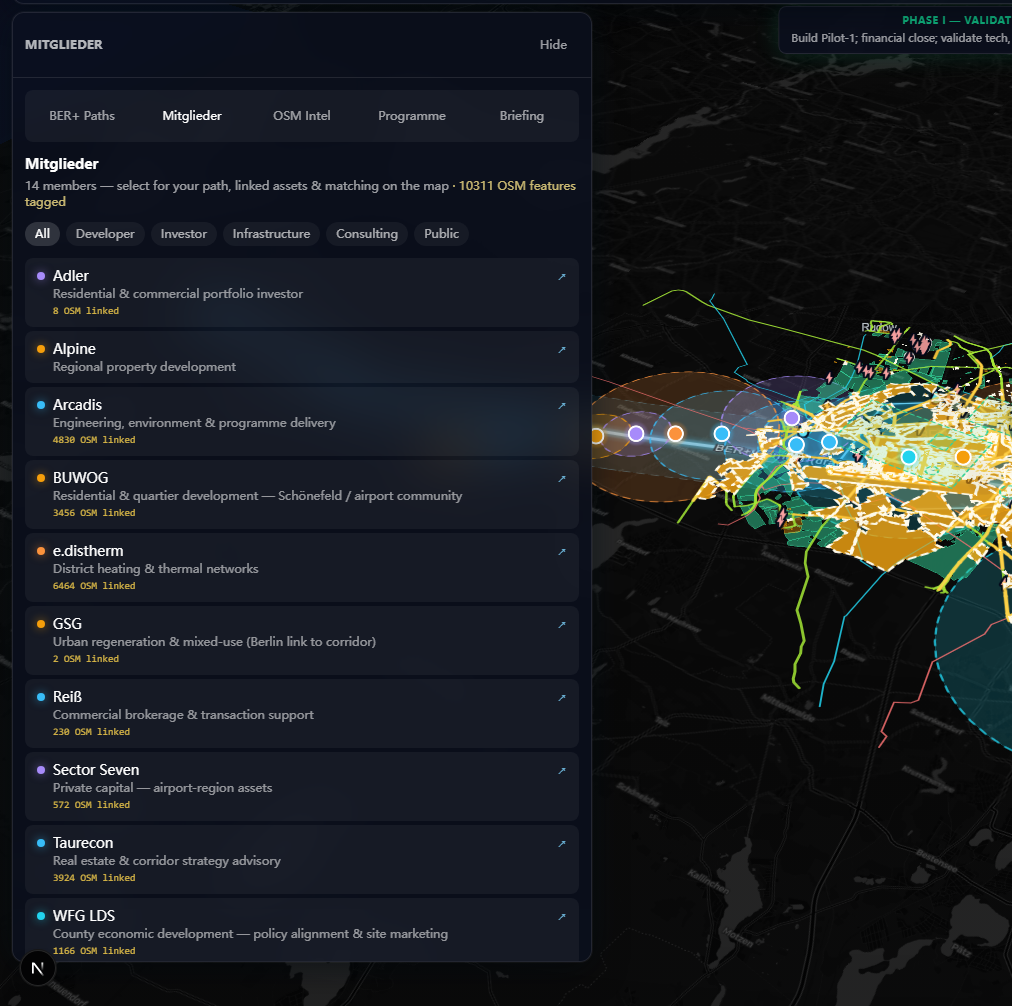
\includegraphics[width=\linewidth,height=0.2\textheight,keepaspectratio]{fig-mitglieder.png}
    \caption*{Mitglieder}
  \end{subfigure}\hfill
  \begin{subfigure}[t]{0.32\textwidth}
    \centering
    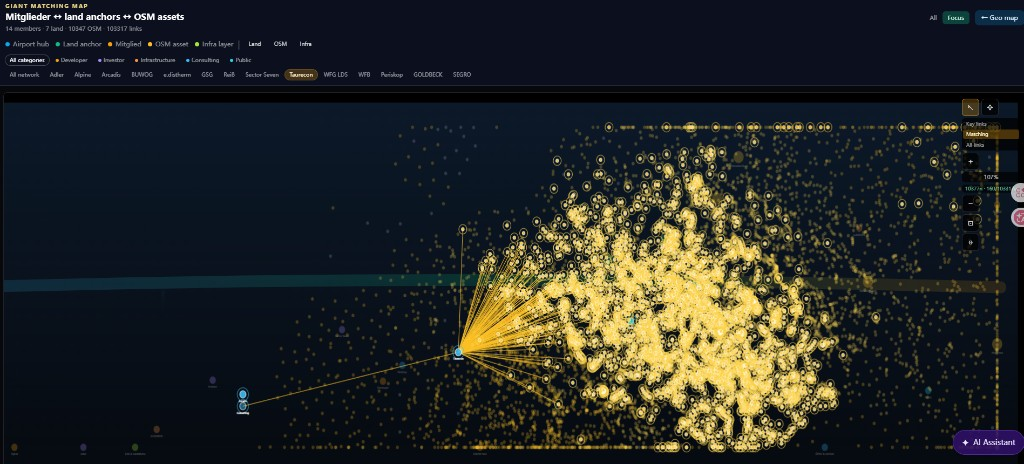
\includegraphics[width=\linewidth,height=0.2\textheight,keepaspectratio]{fig-matching-map.png}
    \caption*{Matching map}
  \end{subfigure}
\end{figure}

\section*{3.\ Stakeholder signal --- Thomas Graf (Alpine Immobilien)}
\textbf{Context.} After the June presentation, \textbf{Thomas Graf} (Geschäftsführer, Alpine Immobilien GmbH; BER+ 2.\ Vorsitzender; developer of the BB Business Hub, Schönefeld) asked about \textbf{employee numbers} of firms near Schönefeld --- whether a new project there would have enough ``manpower'' to succeed.

\textbf{Reframing (EN / DE).}
\begin{itemize}
  \setlength{\itemsep}{0.12em}
  \item \textbf{Not} primarily: construction or factory labour on site.
  \item \textbf{Rather:} \textit{Beschäftigungstiefe} --- how many jobs and firms already exist; can new \textbf{Büro/Gewerbe} attract tenants; can those tenants recruit \textbf{Fachkräfte} in the corridor (Alpine's core leasing question).
\end{itemize}

Graf himself cites the campus proof point: \textbf{$\sim$50 companies, $\sim$800 employees} at BB Business Hub (BER+ news, Feb 2025). The 2025 \textbf{FBB/WFBB/IHK} Flughafenregion labour study notes strong employment growth but \textbf{Fachkräftegewinnung} as the top business challenge --- mobility and the wider Berlin--Brandenburg catchment ($\sim$6\,M) matter as much as local headcount.

\textbf{Board Room response.} Show Mitglieder, gewerbe/OSM layers, and corridor links on one map; label data \textit{indicative}. Verified firm-level \textbf{Beschäftigtenzahlen} would need a BER+ member validation pass (pilot: Alpine + 3--5 anchor Mitglieder) --- transparency before strategy, not a finished labour-market GIS.

\section*{4.\ What BER+ must run (pilot phase)}
BER+ must \textbf{collect} member data, \textbf{validate} locations, \textbf{define} ownership \& refresh rules, \textbf{maintain} quarterly OSM snapshots, and \textbf{host} the neutral Board Room. Phase I anchors on Pilot-1 (SEGRO / Schönefeld Nord).

\section*{5.\ Team recommendations}
\textbf{Pursue:} host Board Room as briefing surface; pilot 3--5 verified member--asset links; quarterly OSM refresh; Inquiry Ledger from matching ``Save''.

\textbf{Deprioritize:} cadastral GIS replacement; single-member walled gardens; unverified claims as authoritative.

\textbf{Next step (90 days):} board MOU for hosting + one recorded briefing with a Pilot-1 decision on the shared map.

\sectionrule
{\small
\textbf{Sources:} OSM via \texttt{/api/osm/schoenefeld}; benchmarks (Amsterdam Airport City; Schiphol AAA / ISOCARP 2021; VLAIO / Geopunt); BER+ member materials; Thomas Graf / Alpine (BER+ Koepfe interview; BB Business Hub news); FBB/WFBB/IHK labour study Flughafenregion 2025.\\
Map figures: curated app captures (\texttt{docs/presentation/figures}); welcome screen: Playwright E2E.
}

\end{document}
